\part{Approximation Methods}
    \section{Time Independent, Non-Degenerate, Perturbation Theory}
    Many problems in quantum mechanics cannot be solved analytically.
    In these cases often the best we can do is approximate.
    One of the principle ways that we do this is we try to treat the unsolvable problem as a solvable problem with an extra term.
    This is done by defining the Hamiltonian
    \[\operator{H} = \operator{H}_0 + \operator{H}'\]
    where \(\operator{H}_0\) is the Hamiltonian for a system which we can solve exactly and \(\operator{H}'\), known as the perturbation Hamiltonian, is a `small' (exactly what we mean by small will be made clear later) perturbation.
    
    Since the \gls{tise} can be solved exactly for \(\operator{H}_0\) we assume that the eigenvalues, \(\{E_{n}^{(0)}\}\), are known as well as the corresponding eigenstates, \(\{n^{(0)}\}\).
    The aim is to find the eigenvalues and eigenstates of \(\operator{H}\).
    Since \(\operator{H}'\) is `small' we expect these to be close to the eigenvalues and eigenstates of \(\operator{H}_0\).
    
    As with many other problems when we have to approximate we attempt a solution in the term of a series.
    We introduce a parameter, \(\lambda\), which allows us to keep track of powers of \(\operator{H}'\):
    \[\operator{H} = \operator{H}_0 + \lambda\operator{H}'.\]
    This parameter will be set to one later on.
    
    We will assume that the eigenstates of \(\operator{H}\) and \(\operator{H}_0\) are discrete.
    We will also assume that the eigenstates \(\ket{n^{(0)}}\) are non-degenerate and therefore all uniquely identified by their energy.
    In later sections we will look at what happens if \(\ket{n^{(0)}}\) aren't degenerate or \(\operator{H}'\) is time dependent.
    
    Currently we know that
    \[\operator{H}_0\ket{n^{(0)}} = E_n^{(0)}\ket{n^{(0)}}.\]
    The goal is, as usual, to solve the \gls{tise} for \(\operator{H}\):
    \[\operator{H}\ket{n} = E_n\ket{n}.\]
    We assume that \(E_n\) and \(\ket{n}\) can be expanded in a series:
    \begin{align*}
        E_n &= E_n^{(0)} + \lambda E_n^{(1)} + \lambda E_n^{(2)} + \dotsb\\
        \ket{n} &+ \ket{n^{(0)}} + \lambda\ket{n^{(1)}} + \lambda^2\ket{n^{(2)}} + \dotsb
    \end{align*}
    Where the correction terms, \(E^{(i)}\) and \(\ket{n^{(i)}}\), \(i \ge 1\), are of successively smaller size.
    We keep track of this with \(\lambda\) but remember that \(\lambda\) will be set to one so it is not actually controlling the size.
    Notice also that the correction terms, \(\ket{n^{(i)}}\), are not normalised.
    
    Substituting these series into the \gls{tise} we get
    \begin{align*}
        \operator{H}\ket{n} &= (\operator{H}_0 + \lambda\operator{H}')\ket{n}\\
        &= (\operator{H}_0 + \lambda\operator{H}')(\ket{n^{(0)}} + \lambda\ket{n^{(1)}} + \lambda^2\ket{n^{(2)}} + \dotsb)\\
        &= (E_n^{(0)} + \lambda E_n^{(1)} + \lambda^2E_n^{(2)} + \dotsb)(\ket{n^{(0)}} + \lambda\ket{n^{(1)}} + \lambda^2\ket{n^{(2)}} + \dotsb).
    \end{align*}
    Equating terms of the same order in \(\lambda\) we see that
    \begin{align*}
        \lambda^0: && \operator{H}_0\ket{n^{(0)}} &= E_n^{(0)}\ket{n^{(0)}}\\
        \lambda^1: && \operator{H}_0\ket{n^{(1)}} + \operator{H}'\ket{n^{(0)}} &= E_n^{(0)}\ket{n^{(1)}} + E_n^{(1)}\ket{n^{(0)}}\\
        \lambda^2: && \operator{H}_0\ket{n^{(2)}} + \operator{H}'\ket{n^{(1)}} &= E_n^{(0)}\ket{n^{(2)}} + E_n^{(1)}\ket{n^{(1)}} + E_n^{(2)}\ket{n^{(0)}}.
    \end{align*}
    Collecting terms by state these become
    \begin{align*}
        \lambda^0: && \operator{H}_0\ket{n^{(0)}} &= E_n^{(0)}\ket{n^{(0)}}\\
        \lambda^1: && (\operator{H}_0 - E_n^{(0)})\ket{n^{(1)}} &= (E_n^{(1)} - \operator{H}')\ket{n^{(0)}}\\
        \lambda^2: && (\operator{H}_0 - E_n^{(0)})\ket{n^{(2)}} &= (E_n^{(1)} - \operator{H}')\ket{n^{(1)}} + E_n^{(2)}\ket{n^{(0)}}.
    \end{align*}
    The first of these, \(\lambda^0\), tells us nothing new, it is simply a restatement of \(\ket{n^{(0)}}\) as an eigenstate of \(\operator{H}_0\).
    
    Considering the first order terms take an inner product with the \(k\)th unperturbed eigenstate:
    \begin{equation}\label{eqn:first order correction}
        \bra{k^{(0)}}(\operator{H}_0 - E_n^{(0)})\ket{n^{(1)}} = 	\bra{k^{(0)}}(E_n^{(1)} - \operator{H}')\ket{n^{(0)}}.
    \end{equation}
    The first term of the left hand side gives us
    \begin{align*}
        \bra{k^{(0)}}\operator{H}_0\ket{n^{(1)}} &= \bra{n^{(1)}}\operator{H}_0\hermit \ket{k^{(0)}}^*\\
        &= \bra{n^{(1)}}\operator{H}_0\ket{k^{(0)}}^*\\
        &= E_k^{(0)}\braket{n^{(1)}}{k^{(0)}}^*\\
        &= E_k^{(0)}\braket{k^{(0)}}{n^{(1)}}.
    \end{align*}
    Thus equation~\ref{eqn:first order correction} becomes
    \[(E_k^{(0)} - E_n^{(0)})\braket{k^{(0)}}{n^{(1)}} = E_n^{(1)}\delta_{kn} - \bra{k^{(0)}}\operator{H}'\ket{n^{(0)}}.\]
    We chose \(k\) to be arbitrary, we now choose \(k = n\) and this becomes
    \[0 = E_n^{(1)} - H_{nn}\]
    
    \[
        \tcbhighmath{\Delta E^{(1)} = E_n^{(1)} = H_{nn} = \bra{n^{(0)}}\operator{H}'\ket{n^{(0)}}.}
    \]
    
    This tells us the shift in the energy of the \(n\)th eigenvalue to first order.
    In words this tells us: the shift in energy induced by a perturbation is given to first order by the expectation value of the perturbation with respect to the unperturbed state.
    
    Since \(E_n^{(1)}\) represents the shift in energy to first order it is sometimes written as \(\Delta E_n^{(1)}\) or \(\Delta E_n\).
    \begin{figure}[ht]
        \centering
        \tikzsetnextfilename{first-order-energy-shift}
        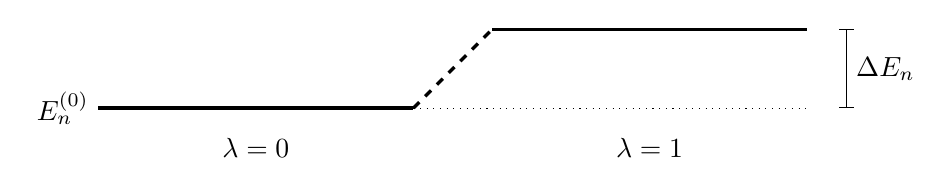
\begin{tikzpicture}
            \tikzstyle{energy level} = [very thick]
            \draw[energy level] (0, 0) -- (4, 0);
            \draw[energy level] (5, 1) -- (9, 1);
            \draw[dashed, energy level] (4, 0) -- (5, 1);
            \draw[dotted] (4, 0) -- (9, 0);
            \node[left] at (0, 0) {\(E_n^{(0)}\)};
            \draw[|-|] (9.5, 0) -- (9.5, 1);
            \node[right] at (9.5, 0.5) {\(\Delta E_n\)};
            \node at (2, -0.5) {\(\lambda = 0\)};
            \node at (7, -0.5) {\(\lambda = 1\)};
        \end{tikzpicture}
        \caption{The first order effect of a perturbation on a non-degenerate energy level of energy \(E_n^{(0)}\).}
    \end{figure}
    If instead we choose \(k \ne n\) then we have
    \[(E_k^{(0)} - E_n^{(0)})\braket{k^{(0)}}{n^{(1)}} = -\bra{k^{(0)}} \operator{H}' \ket{n^{(0)}}, \qquad k\ne n.\]
    Since \(\ket{n^{(1)}}\) is just a state it can be expanded in terms of the unperturbed eigenbasis:
    \[\ket{n^{(1)}} = \sum_{m} c_{nm}^{(1)}\ket{m^{(0)}}.\]
    Taking an inner product with \(\bra{k^{(0)}}\) we find
    \begin{align*}
        \braket{k^{(0)}}{n^{(0)}} &= \sum_m c_{nm}^{(1)}\braket{k^{(0)}}{m^{(0)}}\\
        &= \sum_{m} c_{nm}^{(1)}\delta_{km}\\
        &= c_{nk}^{(1)}.
    \end{align*}
    Hence
    \[(E_k^{(0)} - E_n^{(0)})c_{nk}^{(1)} = -\bra{k^{(0)}}\operator{H}' \ket{n^{(0)}} \implies c_{nk}^{(1)} = \frac{\bra{k^{(0)}} \operator{H'} \ket{n^{(0)}}}{E_n^{(0)} - E_k^{(0)}} = \frac{H'_{kn}}{E_n^{(0)} - E_k^{(0)}}, \qquad k \ne n.\]
    So we have now determined all of the coordinates of \(\ket{n^{(0)}}\) apart from \(c_{nn}^{(1)}\).
    However it turns out that if we choose the correction terms to be orthogonal to the unperturbed states then \(c_{nn}^{(1)} = 0\).
    Thus we have fully specified \(\ket{n^{(1)}}\) in the \(\{\ket{k^{(0)}}\}\) basis and we find that
    \[
        \tcbhighmath{\ket{n^{(1)}} = \sum_{k\ne n} \frac{\bra{k^{(0)}} \operator{H} \ket{n^{(0)}}}{E_n^{(0)} - E_k^{(0)}}\ket{k^{(0)}} = \sum_{k\ne n}\frac{H'_{kn}}{E_n^{(0)} - E_k^{(0)}}\ket{k^{(0)}}.}
    \]
    We say that the perturbation mixes the unperturbed states since the perturbed states have a small component from each unperturbed state.
    Unlike with the energy shift we have a potentially infinite sum to evaluate.
    This, along with the initial assumption that the series expansions exist, means that several things have to be `small':
    \begin{itemize}
        \item For first order changes to the eigenstate to be small we require
        \[\abs*{H'_{kn}} \ll \abs*{E_n^{(0)} - E_k^{(0)}} \forall k\ne n.\]
        \item For first order changes to the energy levels to be small we require
        \[\abs*{E_n^{(1)}} \ll \min \left\{ \abs*{E_n^{(0)}} - E_{k}^{(0)} \right\}.\]
    \end{itemize}
    Note that these conditions break down if there is degeneracy in the unperturbed system, for example some terms of the sum for \(\ket{n^{(1)}}\) will become undefined if \(E_k^{(0)} = E_n^{(0)}\) for \(k \ne n\).
    However we only need the particular energy level for the shift that we are calculating to be non-degenerate for this analysis to be correct.
    Other energy levels can be degenerate but we will need to treat them specially when we come to calculate their energy shift.
    
    \begin{example}
        \textit{Consider the potential}
        \[
            V(x) =
            \begin{cases}
                V_0\cos\left(\frac{\pi x}{2a}\right), & \abs{x} \le a,\\
                \infty, & \abs{x} > a.
            \end{cases}
        \]
        \textit{Calculate the ground state energy to first order in perturbation theory.}
        This corresponds to an infinite square well with the floor of the well bulging upwards in the centre.
        We can consider the Hamiltonian for this system to be the Hamiltonian for the square well plus a perturbative cosine term.
        We already know the solutions for the infinite square well:
        \begin{align*}
            E_n^{(0)} &= \frac{\pi^2\hbar^2n^2}{8ma^2},\\
            u_n^{(0)}(x) &= \frac{1}{\sqrt{a}}\cos\left(\frac{n\pi x}{2a}\right), \qquad n~\text{odd},\\
            u_n^{(0)}(x) &= \frac{1}{\sqrt{a}}\sin\left(\frac{n\pi x}{2a}\right), \qquad n~\text{even},\\
        \end{align*}
        The perturbation is then
        \[\operator{H}' = V_0\cos\left(\frac{\pi x}{2a}\right).\]
        This is `small' as long as \(V_0 \ll E_2^{(0)} - E_1^{(0)}\).
        The first order correction to the energy is then
        \[\Delta E = E_1^{(1)} = H'_{11} = \int_{-\infty}^{\infty} u_1^{(0)}\operator{H'}u_1^{(0)}\dd{x} = \frac{V_0}{a} \int_{-a}^{a} \cos^3\left(\frac{\pi x}{2a}\right) \dd{x} = \frac{8V_0}{3\pi} \approx 0.85V_0.\]
    \end{example}
    
    \subsection{Higher Orders}
    Sometimes the first order correction is zero.
    If this is the case then we need to go to second order.
    Going back to the result for the second order terms in \(\lambda\) we had
    \[(\operator{H}_0 - E_n^{(0)})\ket{n^{(2)}} = (E_n^{(1)} - \operator{H}')\ket{n^{(1)}} + E_n^{(2)}\ket{n^{(0)}}.\]
    Taking an inner product with an unperturbed eigenstate gives
    \[\bra{k^{(0)}}(\operator{H}_0 - E_n^{0})\ket{n^{(2)}} = \bra{k^{(0)}}(E_n^{(1)} - \operator{H}')\ket{n^{(1)}} + E_n^{(2)}\delta_{kn}.\]
    As before the first term on the left hand side can be shown to be \(E_{k}^{(0)}\braket{k^{(0)}}{n^{(2)}}\) so
    \[(E_k^{(0)} - E_{n}^{(0)})\braket{k^{(0)}}{n^{(2)}} = \bra{k^{(0)}}(E_n^{(1)} - \operator{H}')\ket{n^{(1)}} + E_n^{(2)}\delta_{kn}.\]
    In the case that \(k = n\) we find that
    \begin{align*}
        E_n^{(2)} &= \bra{n^{(0)}}\operator{H}'\ket{n^{(1)}} - E_n^{(1)}\braket{n^{(0)}}{n^{(1)}}
        \shortintertext{we choose the perturbative term \(\ket{n^{(1)}}\) to be orthogonal to the eigenstate \(\ket{n^{(0)}}\) leaving}
        &= \bra{n^{(0)}}\operator{H}'\ket{n^{(1)}}\\
        &= \sum_{m\ne n} c_{nm}^{(1)}\bra{n^0}\operator{H}'\ket{m^{(0)}}\\
        &= \sum_{m\ne n} c_{nm}^{(1)}H'_{nm}\\
        &= \sum_{m\ne n} \frac{H'_{mn}H'_{nm}}{E_n^{(0)} - E_m^{(0)}}\\
        &= \sum_{m\ne n} \frac{\abs{H'_{mn}}}{E_n^{(0)} - E_n^{(0)}}.
    \end{align*}
    Here we have used the expansion of \(\ket{n^{(1)}}\) in the \(\{\ket{m^{(0)}}\}\) eigenbasis, the formula we found for \(c_{nm}^{(1)}\), and the fact that \(H'\) is Hermitian so \(H'_{nm} = H'^*_{nm}\).
    
    We see that for the second order energy shift we have to calculate an infinite sum.
    To find the second order correction to the state we would need a double infinite sum and so on.
    Sometimes symmetry dictates that only a finite number of terms will be non-zero, sometimes we just have to truncate the sum after some number of terms.
    
    \subsection{Convergence}
    \textit{This section is non-examinable.}
    
    The series expansions that we come up with in perturbation theory often aren't actually convergent.
    This is because even though each term is small each correction contains multiple infinite sums which dominate and cause the series to diverge.
    Formally these series are asymptotic series.
    An asymptotic series for \(f\) is a series whose partial sums, that is the sum up to and including the \(n\)th term, evaluated at \(x\) can be made arbitrarily close to \(f(x)\) by taking sufficiently large \(x\).
    This differs from the usual definition of a convergent sum where the sequence of \(n\)th partial sums tends to \(f(x)\) as \(n\to\infty\) for all \(x\).
    
    \section{Degenerate, Time Independent, Perturbation Theory} 
    Suppose that the unperturbed Hamiltonian, \(\operator{H}_0\), has one eigenvalue which is \(g\)-fold degenerate.
    We label the states such that the first \(g\)-states are degenerate so
    \begin{align*}
        \operator{H}_0\ket{E_n^{(0)}} &= E^{(0)}\ket{E_n^{(0)}}, && n = 1, \dotsc, g,\\
        \operator{H}_0\ket{E_n^{(0)}} &= E_n^{(0)}\ket{E_n^{(0)}}, && n > g.
    \end{align*}
    Here \(E^{(0)}\) is the degenerate eigenvalue and \(E^{(0)} \ne E_n^{(0)}\) for \(n > g\).
    All other energy levels are non-degenerate so \(E_n^{(0)} \ne E_m^{(0)}\) for \(n\ne m\) and \(n, m > g\).
    
    We can choose a basis such that the \(g\) degenerate states are mutually orthogonal.
    Any linear combination of degenerate states, such as
    \[\ket{E^{(0)}} = \sum_{n=1}^g b_n\ket{E_n^{(0)}},\]
    will be another eigenstate of \(\operator{H}_0\) with eigenvalue \(E^{(0)}\).
    
    In the non-degenerate case we assumed that the perturbed eigenstates were close to the unperturbed states.
    More formally there was a one-to-one correspondence between the unperturbed states, \(\{n^{(0)}\}\), and the perturbed states \(\ket{n}\), and it was possible to continuously move from a perturbed state to an unperturbed state by allowing \(\lambda \to 0\).
    This cannot be assumed to be the case for a degenerate system because of the freedom we have in picking the basis for the degenerate subspace.
    In the limit \(\lambda \to 0\) we cannot be sure which of the infinite set of degenerate eigenstates the series will converge to.
    We aim to find a linear combination of eigenstates, \(\{\ket{E^{(0)}}\}\), such that these eigenstates are close to the perturbed states.
    
    As before we start with
    \[(\operator{H}_0 + \lambda\operator{H}')\ket{E} = E\ket{E}\]
    where
    \begin{align*}
        E &= E^{(0)} + \lambda E^{(1)} + \lambda^2E^{(2)} + \dotsb,\\
        \ket{E} &= \ket{E^{(0)}} + \lambda\ket{E^{(1)}} + \lambda^2\ket{E^{(2)}} + \dotsb.
    \end{align*}
    As before by equating coefficients of \(\lambda\) we see that
    \begin{align*}
        \lambda^0: && (\operator{H}_0 - E^{(0)})\ket{E^{(0)}} &= 0,\\
        \lambda^1: && (\operator{H}_0 - E^{(0)})\ket{E^{(1)}} + (\operator{H}' - E^{(1)})\ket{E^{(0)}} &= 0,\\
        \lambda^2: && (\operator{H}_0 - E^{(0)})\ket{E^{(2)}} + (\operator{H}' - E^{(1)})\ket{E^{(1)}} - E^{(2)}\ket{E^{(0)}} &= 0.
    \end{align*}
    The first of these simply restates that \(\ket{E^{(0)}}\) is an eigenstate with eigenvalue \(E^{(0)}\).
    For the second we take an inner product with the \(k\)th unperturbed state:
    \[\bra{E_k^{(0)}}(\operator{H}_0 - E^{(0)})\ket{E^{(1)}} + \bra{E_k^{(0)}}(\operator{H}' - E^{(1)})\ket{E^{(0)}}.\]
    As before we use the fact that \(\bra{E_k^{(0)}}\operator{H}_0 = E_k^{(0)}\bra{E_k^{(0)}}\) for the first term and for the second term we use
    \[\bra{E^{(0)}} = \sum_{n=1}^g b_n\ket{E_n^{(0)}}\]
    to get
    \[(E_k^{(0)} - E^{(0)})\braket{E_k^{(0)}}{E^{(0)}} + \sum_{n=1}^g b_n (H'_{kn} - E^{(1)}\delta_{kn})\]
    where
    \[H'_{kn} = \bra{E_k^{(0)}}\operator{H}'\ket{E_n^{(0)}}, \qquad\text{and}\qquad \braket{E_k^{(0)}}{E_n^{(0)}} = \delta_{kn}.\]
    We chose \(k\) arbitrarily and we now consider the case when \(k \le g\).
    In this case \(E_k^{(0)} = E^{(0)}\) so this equation reduces to
    \[\sum_{n=1}^g (H'_{kn} - E^{(1)}\delta_{kn})b_n = 0, \qquad k = 1, \dotsc, g.\]
    This is simply an eigenvalue problem in the \(g\) dimensional degenerate subspace.
    We can make this more explicit if we define a \(g\times g\) matrix, \(H'\), with components \(H'_{kn}\), and the \(g\)-dimensional identity matrix, \(\ident\), which has components \(\delta_{kn}\).
    Then this equation becomes
    \[(H' - E^{(1)}\ident)\vv{b} = 0\]
    where \(\vv{b}\) is some \(g\)-dimensional eigenvector to be determined.
    
    For this to have non-trivial solutions the determinant must be zero, so
    \[
        \begin{vmatrix}
            H'_{11} - E^{(1)} & H'_{12} & \dots & H'_{1g}\\
            H'_{21} & H'_{22} - E^{(1)} & \dots & H'_{2g}\\
            \vdots & \vdots & \ddots & \vdots\\
            H'_{g1} & H'_{g2} & \dots & H'_{gg} - E^{(1)}
        \end{vmatrix}
        = 0.
    \]
    The determinant is a \(g\) degree polynomial in \(E^{(1)}\) and therefore has \(g\) roots.
    Each root corresponds to a set of coefficients, \(\{b_n\}\).
    The roots are real since \(H'\) is a Hermitian matrix.
    There are three cases that we consider.
    \begin{itemize}
        \item \textit{All roots distinct} -- In this case the \(g\)-fold degeneracy is completely lifted at first order and the degenerate energy level splits into \(g\) distinct levels.
        \item \textit{Some roots equal} -- In this case the \(g\)-fold degeneracy is partly lifted at first order and the degenerate energy level splits into some distinct levels.
        \item \textit{All roots equal} -- In this case the degeneracy remains completely at first order, as long as the roots are non-zero there is still a first order energy shift, it just doesn't separate the energy levels.
    \end{itemize}
    These are shown in figure~\ref{fig:root possibilities}.
    \begin{figure}
        \centering
        \tikzsetnextfilename{degeneracy-breaking}
        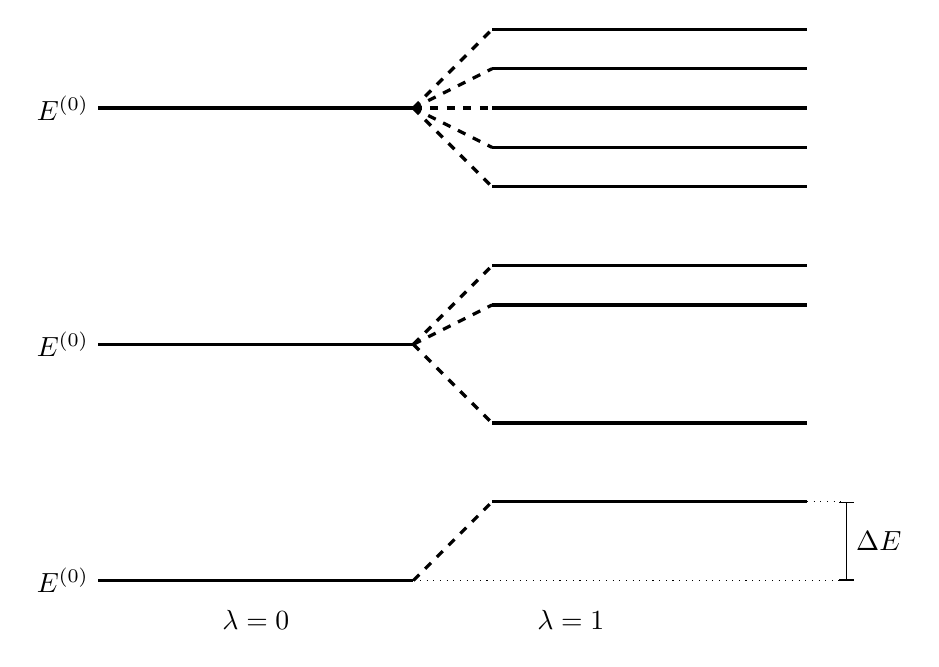
\begin{tikzpicture}
            \tikzstyle{energy level} = [very thick]
            \draw[energy level] (0, 0) -- (4, 0);
            \foreach \y in {1, 0.5, 0, -0.5, -1} {
                \draw[energy level] (5, \y) -- (9, \y);
                \draw[energy level, dashed] (4, 0)  -- (5, \y);
            }
            \node[left] at (0, 0) {\(E^{(0)}\)};
            \begin{scope}[yshift=-3cm]
                \draw[energy level] (0, 0) -- (4, 0);
                \foreach \y in {1, 0.5, -1} {
                    \draw[energy level] (5, \y) -- (9, \y);
                    \draw[energy level, dashed] (4, 0)  -- (5, \y);
                }
                \node[left] at (0, 0) {\(E^{(0)}\)};
            \end{scope}
            \begin{scope}[yshift=-6cm]
                \draw[energy level] (0, 0) -- (4, 0);
                \draw[energy level] (5, 1) -- (9, 1);
                \draw[energy level, dashed] (4, 0)  -- (5, 1);
                \node[left] at (0, 0) {\(E^{(0)}\)};
                \draw[dotted] (4, 0) -- (9.5, 0);
                \draw[dotted] (9, 1) -- (9.5, 1);
                \draw[|-|] (9.5, 0) -- (9.5, 1);
                \node[right] at (9.5, 0.5) {\(\Delta E\)};
                \node at (2, -0.5) {\(\lambda = 0\)};
                \node at (6, -0.5) {\(\lambda = 1\)};
            \end{scope}
        \end{tikzpicture}
        \caption{The three possible cases for roots of the eigenvalue problem with 5-fold degeneracy, top to bottom: all roots distinct, some roots equal, all roots equal.}
        \label{fig:root possibilities}
    \end{figure}
    \subsection{Special Cases}
    For a diagonal matrix the determinant is simply the product along the diagonal.
    If \(H'\) is diagonal then the determinant of \(H' - E^{(1)}\ident\) will be
    \[(H'_{11} - E^{(1)})(H'_{22} - E^{(1)})\dotsm(H'_{gg} - E^{(1)}) = 0\]
    which trivially has roots
    \[\Delta E_n^{(1)} = E^{(0)} = H'_{nn} = \bra{E_n^{(0)}}\operator{H}'\ket{E_n^{(0)}}, \qquad n = 1, \dotsc, g.\]
    We see that this is exactly the same as if \(\operator{H}'\) was non-degenerate.
    Normally to diagonalise a matrix we need to know the eigenvalues and eigenvectors, which requires us to solve the eigenvalue problem so doesn't actually help us solve the eigenvalue problem.
    However here we can use the compatible observables theorem to know that the matrix is diagonal without actually computing it.
    Suppose we can find an observable, \(\observable{A}\), represented by an operator, \(\operator{A}\), such that
    \[[\operator{H}_0, \operator{A}] = [\operator{H}', \operator{A}] = 0.\]
    Notice that this doesn't necessarily mean that \([\operator{H}_0, \operator{H}'] = 0\), in fact we assume this isn't the case as if it was then we wouldn't need perturbation theory.
    We use the fact that \(\operator{H}_0\) and \(\operator{A}\) have a simultaneous eigenbasis, \(\{\ket{E_n^{(0)}, A_i}\}\), and in this basis
    \begin{align*}
        \operator{H}_0\ket{E^{(0)}, A_i} &= E^{(0)}\ket{E^{(0)}, A_i}\\
        \operator{A} \ket{E^{(0)}, A_i} &= A_i \ket{E^{(0)}, A_i}.
    \end{align*}
    If the eigenvalues, \(\{A_i\}\), for \(i = 1, \dotsc, g\), are distinct then we choose these states as our basis states, that is
    \[\ket{E_n^{(0)}} = \ket{E^{(0)}, A_n}, \qquad n = 1, \dotsc, g.\]
    We then use the fact that \(\operator{H}'\) and \(\operator{A}\) commute so
    \[\bra{E_k^{(0)}}[\operator{H}', \operator{A}]\ket{E_n^{(0)}} = 0.\]
    Writing this out in full gives
    \[\bra{E_k^{(0)}}\operator{H}'\operator{A}\ket{E_n^{(0)}} - \bra{E_k^{(0)}}\operator{A}\operator{H}'\ket{E_n^{(0)}} = (A_n - A_k)\bra{E_k^{(0)}}\operator{H}'\ket{E_n^{(0)}} = (A_n - A_k)H'_{kn}.\]
    Since this must always be zero and we assume that \(A_n \ne A_k\) for \(n \ne k\) we must have that \(H'_{kn} = 0\) for \(k \ne n\).
    Thus in this eigenbasis \(\operator{H}'\) is diagonalised and so we can use the same solution as we would for the non-degenerate case.
    
    If \(A_i\) are not distinct then we look for another new operator, \(\operator{B}\), such that \(\{\operator{H}_0, \operator{A}, \operator{B}\}\) and \(\{\operator{H}', \operator{A}, \operator{B}\}\) are mutually commuting sets of operators, and so on.
    
    \begin{example}
        Consider a central potential, \(\operator{V}(r)\), along with spin 1/2 spin-orbit interaction, that is an interaction between the dipole of an electron and the magnetic field it sees due to moving in an electric field.
        The Hamiltonian for this system can be written as
        \[\operator{H} = \frac{\operator{P}^2}{2m} + \operator{V}(r) + f(r)\vecoperator{L}\cdot\vecoperator{S} = \operator{H}_0 + \operator{H'}.\]
        where \(\operator{H}' = f(r)\vecoperator{L}\cdot\vecoperator{S}\).
        Since \(\operator{H}'\) has \(\operator{L}_x\) and \(\operator{S}_x\) components we expect \([\operator{H}', \operator{L}_z] \ne 0 \ne [\operator{H}', \operator{S}_z]\).
        However we do have \([\operator{H}', \operator{J}_z] = 0\) where \(\vecoperator{J} = \vecoperator{L} + \vecoperator{S}\).
        Thus in the coupled basis, \(\ket{n, \ell, s, j, m_j}\), we can use non-degenerate perturbation theory to compute the first order energy shifts.
        Note that \([\operator{H}_0, \vecoperator{L}\cdot\vecoperator{S}] = 0\) but \([\operator{H}_0, \operator{H}']\ne 0\) due to the \(f(r)\) term in \(\operator{H}'\) and the differential operator in \(\operator{H}_0\) due to \(\operator{P}^2 = -\hbar^2\laplacian\).
    \end{example}
    
    \section{Hydrogen Fine Structure}
    As an example of a real life use of perturbation theory we consider the fine structure of hydrogen.
    This results from considering relativistic effects.
    We won't derive these but we will state and explain what they correct for.
    Recall that the unperturbed Hamiltonian for a hydrogen like atom with \(Z\) protons is
    \[\operator{H}_0 = \frac{\operator{P}^2}{2m} + \operator{V}(r), \qquad\text{where}\qquad \operator{V}(r) = -\frac{Ze^2}{4\pi\varepsilon_0r}.\]
    The eigenvalues are given by
    \[E_n^{(0)} = -\frac{m}{2\hbar^2}\left(\frac{Ze^2}{4\pi\varepsilon_0}\right)^2 \frac{1}{n^2} = -\frac{e^2}{2(4\pi\varepsilon_0)a_0}\frac{Z^2}{n^2} = -mc^2\frac{(Z\alpha)}{2n^2}\]
    where \(a_0\) is the Bohr radius and \(\alpha\) is the fine structure constant defined by
    \[a_0 = \frac{4\pi\varepsilon_0\hbar^2}{me^2}, \qquad\text{and}\qquad \alpha = \frac{e^2}{4\pi\varepsilon_0\hbar c} \approx \frac{1}{137}.\]
    One commonly used unit in this context is the rydberg unit of energy defined by
    \[\SI{1}{\rydberg} = \frac{e^2}{2(4\pi\varepsilon_0)a_0} = \SI{13.6}{\electronvolt}.\]
    The ground state of hydrogen is then \(\SI{-1}{\rydberg} = \SI{-13.6}{\electronvolt}\).
    
    \subsection{Perturbed Hamiltonian}
    The perturbation to the Hamiltonian, \(\operator{H}'\), can be further decomposed into three parts:
    \[\operator{H}' = \operator{H}'_{\mathrm{KE}} + \operator{H}'_{\mathrm{SO}} + \operator{H}'_{\mathrm{Darwin}}.\]
    The first term is a relativistic correction to the kinetic energy, which in special relativity is given by \((\gamma - 1)mc^2\).
    Expanding this we see that
    \[(\gamma - 1)mc^2 = \frac{1}{2}mv^2 + \frac{3}{8}m\frac{v^4}{c^2} + \order{v^6}.\]
    For the speeds that an electron travels this fourth order term is small but not entirely negligible.
    It leads to the perturbation
    \[\operator{H}'_{\mathrm{KE}} = -\frac{\operator{P}^4}{8m^3c^2}.\]
    
    The second term is the spin-orbit term which accounts for the interaction between the intrinsic magnetic dipole moment of the electron and the magnetic field that the electron sees due to moving in the electric field created by the nucleus.
    The form of this perturbation is
    \[\operator{H}'_{\mathrm{SO}} = f(r)\vecoperator{L}\cdot\vecoperator{S}\]
    where
    \[f(r) = \frac{2}{m^2c^2r}\dv{V}{r}.\]
    
    The third term, known as the Darwin term\footnote{Named after Charles Galton Darwin who was the grandson of Charles Robert Darwin of evolution fame.} is a relativistic correction to the potential energy given by
    \[\operator{H}'_{\mathrm{Darwin}} = \frac{\hbar^2}{8m^2c^2}\laplacian V(\vv{r}) = \frac{\pi\hbar^2}{2m^2c^2}\frac{Ze^2}{4\pi\varepsilon_0}\delta(\vv{r})\]
    where \(\delta\) is the Dirac delta distribution.
    
    \subsection{Kinetic Energy Correction}
    The unperturbed energy level \(E_n^{(0)}\) for some specific \(n\) is \(2n^2\)-fold degenerate.
    However since \(\operator{H}'_{\mathrm{KE}}\) contains no spin components we know it commutes with \(\operator{S}^2\) and \(\operator{S}_z\).
    It can also be shown that \(\operator{H}'_{\mathrm{KE}}\) commutes with \(\operator{L}^2\) and \(\operator{L}_z\).
    Therefore in the uncoupled basis, \(\{\ket{n, \ell, m_\ell, s, m_s}\}\), \(\operator{H}'_{\mathrm{KE}}\) will be diagonal.
    This means that if we work in the uncoupled basis we can use non-degenerate perturbation theory.
    Since \(\operator{H}'_{\mathrm{KE}}\) has no effect on the spin components we drop \(s\) and \(m_s\) from the notation.
    The first order energy shift is
    \begin{align*}
        \Delta E_{\mathrm{KE}} &= \bra{n, \ell, m_\ell}\left(-\frac{\operator{P}^4}{8m^3c^2}\right)\ket{n, \ell, m_\ell}\\
        &= -\frac{1}{2mc^2}\bra{n, \ell, m_\ell}\operator{T}^2\ket{n, \ell, m_\ell}.
    \end{align*}
    Here we have used the fact that
    \[\operator{T} = \frac{\operator{P}^2}{2m} \implies \operator{T}^2 = \frac{\operator{P}^4}{4m^2}.\]
    Rather than try to compute the fourth derivative, \(\laplacian\laplacian \Psi(\vv{r})\), we use the fact that \(\operator{T} = \operator{H}_0 - \operator{V}(r)\) and therefore
    \[\operator{T}^2 = \operator{H}_0^2 - \operator{H}_0\operator{V}(r) - \operator{V}(r)\operator{H}_0 + \operator{V}(r)\]
    and then \(\Delta E_{\mathrm{KE}}\) is proportional to the expectation value of this:
    \[\Delta E_{\mathrm{KE}} = -\frac{1}{2mc^2}({E_n^{(0)}}^2 - 2E_n^{(0)}\expected{\operator{V}}_{n\ell m_\ell} + \expected{\operator{V}^2}_{n\ell m_\ell}).\]
    Since \(\operator{V} \propto 1/r\) to evaluate the right hand side we simply need \(\expected{1/r}\) and \(\expected{1/r^2}\) which can be shown to be
    \[\expectedResize{\frac{1}{r}}_{n} = \frac{Z}{a_0}\frac{1}{n^2}, \qquad\text{and}\qquad \expectedResize{\frac{1}{r^2}}_{n\ell} = \frac{Z^2}{a_0^2}\frac{1}{n^3(\ell + 1/2)}.\]
    So we find that
    \[\Delta E_{\mathrm{KE}} = -E_n^{(0)}\frac{(Z\alpha)^2}{n^2}\left[\frac{3}{4} - \frac{n}{\ell + 1/2}\right].\]
    As a quick sanity check we see that this is proportional to \(\alpha^2E_n^{(0)} \approx \num{5e-5}E_n^{(0)}\) so the energy shift is indeed small compared to the size of the energy levels, \(E_n^{(0)}\).
    
    \subsection{Spin-Orbit Correction}
    For given values of \(n\) and \(\ell\) the \(E_n^{(0)}\) energy level is \(2(2\ell + 1)\)-fold degenerate.
    This is due to the \(2\ell + 1\) different values of \(m_\ell\) for each value of \(\ell\) and the two possible values of \(m_s\), i.e. \(\pm 1/2\).
    
    However if we work in the coupled basis, \(\{n,\ell, s, j, m_j\}\), then we can use non-degenerate theory.
    To see that this is valid first note that
    \[\operator{H}'_{\mathrm{SO}} = f(r)\vecoperator{L}\cdot\vecoperator{S} = \frac{1}{2}f(r)[\operator{J}^2 - \operator{L}^2 - \operator{S}^2]\]
    and
    \[[\operator{J}^2 - \operator{L}^2 - \operator{S}^2]\ket{n, \ell, s, j, m_j} = [j(j + 1) - \ell(\ell + 1) - s(s + 1)]\hbar^2\ket{n, \ell, s, j, m_j}.\]
    Since this is just an eigenvalue equation we see that \(\operator{H}'_{\mathrm{SO}}\) is diagonal in the coupled basis.
    Thus the energy shift is simply the expectation value in this basis:
    \begin{align*}
        \Delta E_{\mathrm{SO}} &= \bra{n, \ell, s, j, m_j} \operator{H}'_{\mathrm{SO}}\ket{n, \ell, s, j, m_j}\\
        &= \frac{1}{2}[j(j + 1) - \ell(\ell + 1) - s(s + 1)]\hbar^2\expected{f(r)}.
    \end{align*}
    This simplifies since we are considering an electron we know that \(s = 1/2\) and by the angular momentum addition theorem this means that for a given value of \(\ell\)  we have \(j = \ell + 1/2\) or \(j = \ell - 1/2\).
    This means that a state of given \(n\) and \(\ell\) is split into a doublet by the spin-orbit interaction.
    Since \(f(r)\) is independent of \(\vartheta\) and \(\varphi\) and of the spin the expectation value can be written as
    \[\expected{f(r)} = \frac{1}{2m^2c^2}\frac{Ze^2}{4\pi\varepsilon_0}\int_0^{\infty} \frac{1}{r^3}\abs{R_{n\ell}(r)}^2r^2\dd{r}.\]
    Note that the \(1/r^3\) comes from \(f\) and the \(r^2\) comes from the integration measure in polar coordinates.
    It can be shown that
    \[\expectedResize{\frac{1}{r^3}}_{n\ell} = \frac{Z^3}{a_0^3}\frac{1}{n^3\ell(\ell + 1/2)(\ell + 1)}.\]
    For \(\ell \ne 0\) we then find
    \[\Delta E_{\mathrm{SO}} =
        \begin{cases}
            -E_n^{(0)}\frac{(Z\alpha)^2}{2n}\frac{\ell}{\ell(\ell + 1/2)(\ell + 1)}, & j = \ell + \frac{1}{2},\\
            E_n^{(0)}\frac{(Z\alpha)^2}{2n}\frac{1}{\ell(\ell + 1/2)}, & j = \ell - \frac{1}{2}.
        \end{cases}
    \]
    
    \subsection{Darwin Correction}
    The Darwin correction is non-zero only at \(\vv{r} = \vv{0}\) as it is proportional to \(\delta(\vv{r})\).
    The radial function, \(R_{n\ell}(r)\), vanishes at the origin when \(\ell \ne 0\).
    Therefore we only need to consider this term at the origin when \(\ell = 0\) and consequently \(m_\ell = 0\).
    This term also contains no spin components so has no effect on the spin so again we drop \(s\) and \(m_s\) from the notation.
    We find that
    \begin{align*}
        \Delta E_{\mathrm{Darwin}} &= \frac{\pi\hbar^2}{2m^2c^2}\frac{Ze^2}{4\pi\varepsilon_0}\bra{n, 0, 0}\delta(\vv{r})\ket{n, 0, 0}\\
        &= \frac{\pi\hbar^2}{2m^2c^2}\frac{Ze^2}{4\pi\varepsilon_0}\int u_{n00}^*(\vv{r})\delta(\vv{r})u_{n00} \dd[3]{r}\\
        &= \frac{\pi\hbar^2}{2m^2c^2}\frac{Ze^2}{4\pi\varepsilon_0}\abs{u_{n00}(\vv{0})}^2
    \end{align*}
    where in the last step we used the sifting property of the Dirac delta distribution.
    This simplifies as
    \[\abs{u_{n00}(\vv{0})} = \abs{Y_0^0(\vartheta, \varphi)}^2\abs{R_{n\ell}(0)}^2 = \frac{1}{4\pi}\abs{R_{n\ell}(0)}^2 = \frac{Z^3}{\pi a_0^3n^3}.\]
    Hence
    \[\Delta E_{\mathrm{Darwin}} = -E_n^{(0)}\frac{(Z\alpha)^2}{n}.\]
    
    \subsection{Total Correction}
    Combining all three terms it can be shown that
    \[\Delta E_{nj} = E_n^{(0)}\frac{(Z\alpha)^2}{n^2}\left[\frac{n}{j + 1/2} - \frac{3}{4}\right].\]
    
    \begin{figure}[ht]
        \centering
        \tikzsetnextfilename{hydrogen-fine-structure}
        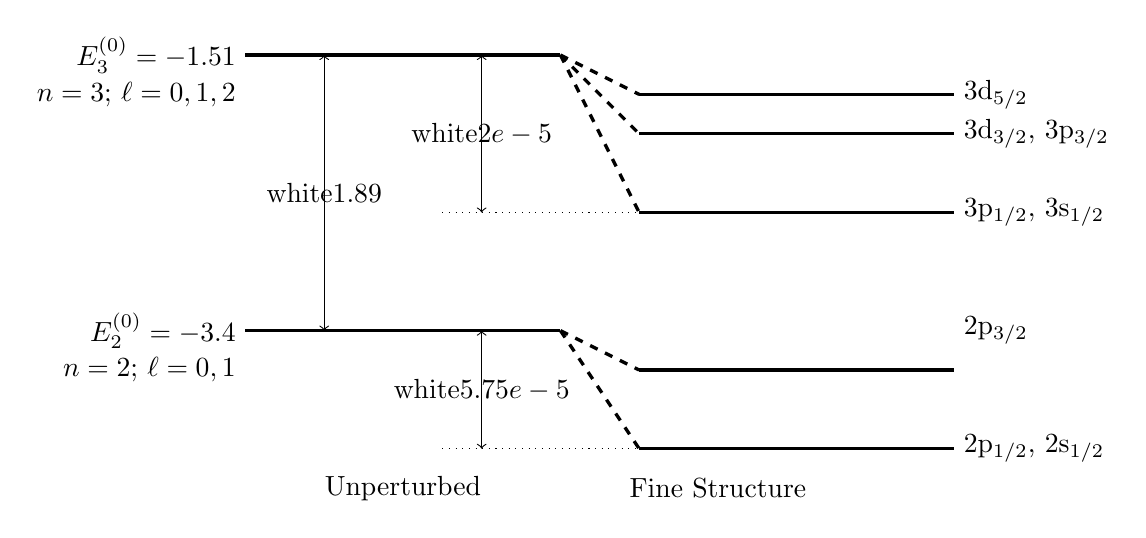
\begin{tikzpicture}
            \tikzstyle{energy level} = [very thick]
            \draw[energy level] (0, 5) -- (4, 5);
            \foreach \y in {4.5, 4, 3} {
                \draw[energy level] (5, \y) -- (9, \y);
                \draw[energy level, dashed] (4, 5) -- (5, \y);
            }
            \draw[energy level] (0, 1.5) -- (4, 1.5);
            \foreach \y in {1, 0} {
                \draw[energy level] (5, \y) -- (9, \y);
                \draw[energy level, dashed] (4, 1.5) -- (5, \y);
            }
            \node[left] at (0, 5) {\(E_3^{(0)} = \SI{-1.51}{\electronvolt}\)};
            \node[left] at (0, 1.5) {\(E_2^{(0)} = \SI{-3.4}{\electronvolt}\)};
            
            \node[right] at (9, 4.5) {\(3\mathrm{d}_{5/2}\)};
            \node[right] at (9, 4) {\(3\mathrm{d}_{3/2}\), \(3\mathrm{p}_{3/2}\)};
            \node[right] at (9, 3) {\(3\mathrm{p}_{1/2}\), \(3\mathrm{s}_{1/2}\)};
            \node[right] at (9, 1.5) {\(2\mathrm{p}_{3/2}\)};
            \node[right] at (9, 0) {\(2\mathrm{p}_{1/2}\), \(2\mathrm{s}_{1/2}\)};
            
            \contourlength{1pt}
            \contournumber{32}
            \draw[<->] (1, 5) -- (1, 1.5) node[midway] {\contour{white}{\(\SI{1.89}{\electronvolt}\)}};
            \draw[dotted] (2.5, 3) -- (5, 3);
            \draw[<->] (3, 3) -- (3, 5) node[midway] {\contour{white}{\(\SI{2e-5}{\electronvolt}\)}};
            \draw[dotted] (2.5, 0) -- (5, 0);
            \draw[<->] (3, 0) -- (3, 1.5) node[midway] {\contour{white}{\(\SI{5.75e-5}{\electronvolt}\)}};
            \node[left] at (0, 4.5) {\(n = 3\); \(\ell = 0, 1, 2\)};
            \node[left] at (0, 1) {\(n = 2\); \(\ell = 0, 1\)};
            \node at (2, -0.5) {Unperturbed};
            \node at (6, -0.5) {Fine Structure};
        \end{tikzpicture}
        \caption{The fine structure of the \(n = 2, 3\) energy levels of hydrogen (not to scale).}
        \label{fig:H fine structure}
    \end{figure}
    The resulting energy levels that occur when we account for relativistic effects are shown (not to scale) in figure~\ref{fig:H fine structure}.
    Since \(\Delta E \propto \alpha^2\) the energy shifts are therefore on the order of \(\SI{e-4}{\electronvolt}\).
    The degeneracy between the states with \(\ell = j \pm 1/2\), such as \(\termNotation[2]{}{\mathrm{p}}{1/2}\) and \(\termNotation[2]{}{\mathrm{s}}{1/2}\), is lifted if we take into account effects from \gls{qed}.
    This shift, called the Lamb shift, was discovered experimentally in 1947 by Lamb and Rutherford.
    In atomic hydrogen this shift is another two orders of magnitude smaller than the relativistic shifts, on the order of \(\SI{4e-6}{\electronvolt}\).
    
    \subsection{Term Notation}
    Term notation, also know as Russell--Saunders notation is a way of denoting a particular state with orbital angular momentum \(\ell\), spin \(s\), and total angular momentum \(j\).
    Such states are denoted
    \[\termNotation{2s + 1}{l}{j}.\]
    Here \(l\) is a letter corresponding to a particular value of \(\ell\) as given in table~\ref{tab:l letters}
    \begin{table}[ht]
        \centering
        \begin{tabular}{c|cccccccc}
            \(\ell\) & 0 & 1 & 2 & 3 & 4 & 5 & 6 & 7\\\hline
            \(l\)    & s & p & d & f & g & h & i & k
        \end{tabular}
        \caption{The orbital angular momentum quantum number, \(\ell\), and the corresponding letter used in term notation. From \(f\) onwards the letters are simply alphabetical skipping \(\mathrm{j}\). The first few letters come from the names for the corresponding spectral lines, namely sharp, primary, diffuse, and fundamental}
        \label{tab:l letters}
    \end{table}
    If the principle quantum number, \(n\), is important then it is prepended:
    \[\termNotation[n]{2s + 1}{l}{j}.\]
    Since for one electron atoms like hydrogen the spin is always \(s = 1/2\) often the spin is dropped from the notation.
    
    For example the ground state of hydrogen has \(n = 1\), \(\ell = 0\), \(s = 1/2\), and \(j = 1/2\).
    Therefore the corresponding state can be denoted as any of the following:
    \[\termNotation[1]{2}{\mathrm{s}}{1/2}, \qquad \termNotation[1]{}{\mathrm{s}}{1/2}, \qquad \termNotation{2}{\mathrm{s}}{1/2}, \qquad \termNotation{}{\mathrm{s}}{1/2} \qquad\text{or}\qquad \termNotation{}{\mathrm{s}}{}.\]
    
    \section{Helium Atom}
    \subsection{The Hamiltonian}
    Helium, \ce{He}, is the second element on the periodic table.
    It has two protons and two electrons.
    We label these electrons 1 and 2.
    The Hamiltonian for a \ce{He} atom is
    \[\operator{H} = \operator{H}_1 + \operator{H}_2 + \frac{e^2}{4\pi\varepsilon\abs{\vv{r_1} - \vv{r_2}}}\]
    where
    \[\operator{H}_i = \frac{\operator{P}_i^2}{2m} - \frac{2e^2}{4\pi\varepsilon_0}.\]
    This Hamiltonian is the sum of the a Hamiltonian for hydrogen like atom as well as an electron--electron interaction term.
    Notice that the Hamiltonian is symmetric under exchanging of the two electrons.
    That is if we change all the terms labelled 1 to be labelled 2 and vice versa the Hamiltonian wouldn't change.
    This is important as electrons are identical so it should be able to swap them without changing the physics.
    Our goal in this section is to apply perturbation theory to find the energy of the ground state.
    
    \subsection{Electron Wave Functions}
    Before we can apply perturbation theory we need to know the ground state of the unperturbed system.
    We first consider the spin components.
    Recall that since electrons are spin 1/2 particles the entire system is thus a spin 1 system.
    We will use a condensed notation where
    \[\alpha = \ket{\spinUp}, \qquad \beta = \ket{\spinDown}, \qquad \chi_{SM_S} = \ket{s_1 = 1/2, s_2 = 1/2, S, M_S}.\]
    We will also use subscripts for \(\alpha\) and \(\beta\) to denote the electron that the state corresponds to.
    As well as this tensor products will simply be written by putting the two vectors next to each other without the usual \(\tensorProd\) symbol.
    
    Recall that there are three triplet states:
    \[\chi_{11} = \alpha_1\alpha_2, \qquad \chi_{10} = \frac{1}{\sqrt{2}}[\alpha_1\beta_2 + \beta_1\alpha_2], \qquad\text{and}\qquad \chi_{1,-1} = \beta_1\beta_2,\]
    and one singlet state:
    \[\chi_{00} = \frac{1}{\sqrt{2}}[\alpha_1\beta_2 - \beta_1\alpha_2].\]
    Notice the triplet states are symmetric under exchange of the two electrons whereas the singlet state is antisymmetric.
    This is important because the spin statistics theorem tells us that the symmetry of a wave function for the whole system must be antisymmetric under exchange of the two electrons.
    That is
    \[\Psi(1, 2) = \psi(\vv{r_1}, \vv{r_2})\chi = -\Psi(2, 1).\]
    
    We start by treating neglecting the electron--electron Coulomb interaction and consider the system as two independent hydrogenic atoms with \(Z = 2\) which have a combined Hamiltonian
    \[\operator{H}_0 = \operator{H}_1 + \operator{H}_2.\]
    We already know the eigenfunctions for \(\operator{H}_i\) are
    \[\operator{H}_iu_{n_i\ell_im_{\ell_i}}(\vv{r_i}) = E_{n_i}u_{n_i\ell_im_{\ell_i}}(\vv{r_i}).\]
    Since the two Hamiltonians only act on their respective electron's:
    \[\operator{H}_iu_{n_1\ell_1m_{\ell_1}}(\vv{r_1})u_{n_2\ell_2m_{\ell_2}}(\vv{r_2}) = E_{n_i}u_{n_1\ell_1m_{\ell_1}}(\vv{r_1})u_{n_2\ell_2m_{\ell_2}}(\vv{r_2})\]
    wave function the action of the total Hamiltonian on the combined state is simply
    \begin{align*}
        \operator{H}_0 u_{n_1\ell_1m_{\ell_1}}(\vv{r_1})u_{n_2\ell_2m_{\ell_2}}(\vv{r_2}) &= (\operator{H}_1 + \operator{H}_2) u_{n_1\ell_1m_{\ell_1}}(\vv{r_1}) u_{n_2\ell_2m_{\ell_2}}(\vv{r_2})\\
        &= (E_{n_1} + E_{n_2}) u_{n_1\ell_1m_{\ell_1}}(\vv{r_1}) u_{n_2\ell_2m_{\ell_2}}(\vv{r_2})\\
        &= E_n u_{n_1\ell_1m_{\ell_1}}(\vv{r_1}) u_{n_2\ell_2m_{\ell_2}}(\vv{r_2}).
    \end{align*}
    So the energy eigenvalues are given by
    \[E_n = E_{n_1} + E_{n_2}, \qquad\text{where}\qquad E_{n_i} = -\frac{m}{2\hbar^2}\left(\frac{2e^2}{4\pi\varepsilon_0}\right)^2\frac{1}{n_i^2}.\]
    
    \subsection{Unperturbed Ground State}
    We are only interested in the ground state, that is \(n = 1\), which corresponds to both constituent systems also being in their ground states, \(n_i = 1\).
    The energy of the ground state, ignoring the effects of the perturbation, is
    \[E_{n=1} = E_{n_1=1} + E_{n_2=1} = 2E_{n_2=1}.\]
    Now we use the fact that for hydrogen with \(Z = 1\) the ground state energy is \(-\SI{13.6}{\electronvolt}\) and helium has the same form of energy levels but with \(Z = 2\).
    Since \(Z\) appears squared in the energy level we expect \(E_{n_i} = 4\cdot(-\SI{13.6}{\electronvolt})\).
    Thus the total energy of the ground state is
    \[E_n = 2\cdot 4 \cdot (-\SI{13.6}{\electronvolt}) = -\SI{108.8}{\electronvolt}.\]
    Experimentally we actually measure the ground state energy to be \(-\SI{78.957}{\electronvolt}\) which is higher.
    The reason this is higher is the repulsive force between the electrons which we have not yet considered.
    
    The wave function in the ground state has \(n_1 = n_2 = 1\) and \(\ell_1 = \ell_2 = m_{\ell_1} = m_{\ell_2} = 0\) which gives the joint spatial wave function in the ground state
    \[\psi_{\mathrm{GS}}(\vv{r_1}, \vv{r_2}) = u_{100}(\vv{r_1})u_{100}(\vv{r_2}).\]
    At this point we remark that the electronic configuration of \ce{He} is typically denoted \(\termNotation[1]{}{\mathrm{s}}{}^2\) where the 1 refers to the value of \(n\), \(s\) corresponds to \(\ell = 1\) and \(2\) tells us that there are two electrons in this state.
    Notice that the ground state wave function is symmetric under exchange of the electrons and therefore for the total ground state wave function, \(\Psi_{\mathrm{GS}} = \psi_{\mathrm{GS}}\chi_{\mathrm{GS}}\), to be antisymmetric \(\chi_{\mathrm{GS}}\) must be antisymmetric.
    Therefore we conclude that \(\chi_{\mathrm{GS}} = \chi_{00}\) as this is the only antisymmetric spin state.
    The total ground state wave function is then
    \[\ket{\Psi_{\mathrm{GS}}} \representation u_{100}(\vv{r_1})u_{100}(\vv{r_2})\chi_{00}.\]
    
    \subsection{The Perturbation}
    We are now in a position to apply perturbation theory to estimate the ground state energy.
    As usual we start with the Hamiltonian
    \[\operator{H} = \operator{H}_0 + \operator{H}'\]
    where
    \[\operator{H}_0 = \operator{H}_1 + \operator{H}_2, \qquad\text{and}\qquad \operator{H}' = \frac{e^2}{4\pi\varepsilon_0\abs{\vv{r_1}-\vv{r_2}}}.\]
    For brevity of notation let \(r_{12} = \abs{\vv{r_1} - \vv{r_2}}\).
    The first order correction to the ground state is then
    \begin{align*}
        \Delta E_1 &= \bra{\Psi_{\mathrm{GS}}} \operator{H}' \ket{\Psi_{\mathrm{GS}}}\\
        &= \bra{\psi, \chi_{00}} \operator{H}' \ket{\psi, \chi_{00}}\\
        &= (\bra{\psi}\tensorProd\bra{\chi_{00}}) \operator{H}' (\ket{\psi} \tensorProd \ket{\chi_{00}})\\
        &= \bra{\psi}\operator{H}'\ket{\psi} \tensorProd \bra{\chi_{00}} \operator{H}' \ket{\chi_{00}}\\
        &= \bra{\psi}\operator{H}'\ket{\psi} \tensorProd \braket{\chi_{00}}{\chi_{00}}\\
        &= \bra{\psi}\operator{H}'\ket{\psi}
    \end{align*}
    Here we have used the fact that \(\operator{H}'\) has no spin components and therefore doesn't act on \(\ket{\chi_{00}}\) so assuming that \(\ket{\chi_{00}}\) is properly normalised the spin terms become one and we drop them.
    Next we use the full form of the \(\termNotation[1]{}{\mathrm{s}}{}\) electron wave function:
    \[u_{100}(\vv{r}) = \frac{1}{\sqrt{\pi}} \left(\frac{Z}{a_0}\right)^{3/2}e^{-Zr/a_0}.\]
    Which gives the integral
    \[\Delta E_1 = \frac{e^2}{4\pi\varepsilon_0} \left(\frac{Z^3}{\pi a_0^3}\right)^{2} \int \frac{1}{r_{12}} \exp\left[-\frac{2Z(r_1 + r_2)}{a_0}\right] \dd[3]{r_1}\dd[3]{r_2}.\]
    This integral can then be shown to give
    \[\Delta E_1 = \frac{5}{4}Z\,\si{\rydberg} = \frac{5}{2}\,\si{\rydberg} = \SI{34}{\electronvolt}.\]
    So to first order we estimate the ground state energy to be
    \[E_1 = -\SI{108.8}{\electronvolt} + \SI{34}{\electronvolt} = -\SI{74.8}{\electronvolt} = -\SI{5.5}{\rydberg}.\]
    This is respectably close to the measured value of \(-\SI{78.957}{\electronvolt}\).
    
    One thing we do have to consider is if perturbation theory is even valid in this case.
    The perturbation is on the order of \SI{10}{\electronvolt}.
    This is only one order of magnitude smaller than the unperturbed energy which on the order of \SI{100}{\electronvolt}.
    As well as this the fine structure corrections will be on the order of \SI{10}{\electronvolt}.
    One justification for using perturbation theory is simply how close the first order energy is to the experimental value.
    
    \section{Multi-Electron Atoms}
    \subsection{Excited States of Helium}
    Recall that the Hamiltonian for Helium is
    \[\operator{H} = \operator{H_1} + \operator{H_2} + \frac{e^2}{4\pi\varepsilon_0\abs{\vv{r_1} - \vv{r_2}}}\]
    where
    \[\operator{H_i} = \frac{\operator{P}_i^2}{2m} - \frac{2e^2}{4\pi\varepsilon_0r_i}.\]
    Ignoring the electron repulsion term the first excited state for helium corresponds to exciting an electron to the first hydrogen-like excited state.
    That is one of \(n_1\) or \(n_2\) becomes \(2\) and the corresponding angular orbital momentum, \(\ell_i\) becomes 0 or 1.
    The corresponding electron configuration is then 1s2s or 1s2p with \(\ell_i = 0, 1\) respectively.
    
    Since the electrons are indistinguishable it doesn't make sense to say which electron is in the excited state.
    Instead we consider a superposition of each electron in the excited state.
    This allows us to construct the spatial wave function
    \[\psi(\vv{r_1}, \vv{r_2}) = \frac{1}{\sqrt{2}} [u_{2\ell m_\ell}(\vv{r_1})u_{100}(\vv{r_2}) \pm u_{100}(\vv{r_1})u_{2\ell m_\ell}(\vv{r_2})].\]
    This is symmetric if we choose \(+\) and antisymmetric if we choose \(-\).
    From this we can construct overall antisymmetric wave functions, the antisymmetry being dictated by spin statistics:
    \begin{align*}
        \Psi_{LM_LSM_S}^{\text{singlet}}(1, 2) &= \frac{1}{\sqrt{2}} [u_{2\ell m_\ell}(\vv{r_1})u_{100}(\vv{r_2}) + u_{100}(\vv{r_1})u_{2\ell m_\ell}(\vv{r_2})] \tensorProd \chi_{S = 0}\\
        \Psi_{LM_LSM_S}^{\text{triplet}}(1, 2) &= \frac{1}{\sqrt{2}} [u_{2\ell m_\ell}(\vv{r_1})u_{100}(\vv{r_2}) - u_{100}(\vv{r_1})u_{2\ell m_\ell}(\vv{r_2})] \tensorProd \chi_{S=1}
    \end{align*}
    Here \(L\) denotes the total angular momentum quantum number.
    It is \(0\) for the 1s2s state and 1 for the 1s2p state.
    
    We can see the degeneracy of various states by considering all possible combinations of quantum numbers allowed by the angular momentum addition theorem.
    First consider the case \(S = 0\).
    There are two options for \(L\), it can be 0 or 1.
    Recall that by the addition of angular momentum theorem the total angular momentum number, \(J\), can be any value from \(L + S\) to \(\abs{L - S}\) decreasing in integer steps.
    The degeneracy, \(g_J\), of this state is then \(2J + 1\).
    The possible values of the quantum numbers the first two excited states are given in table~\ref{tab:degeneracy of helium excited states}.
    \begin{table}[ht]
        \centering
        \begin{tabular}{c|ccc|c}
            \hline
            \(S\) & \(L\) & \(J\) & \(g_J\) &           Terms           \\ \hline
              0   &   0   &   0   &    1    & \(\termNotation{1}{S}{0}\)\\
                  &   1   &   1   &    3    & \(\termNotation{1}{P}{1}\)\\ \hline
              1   &   0   &   1   &    3    & \(\termNotation{3}{S}{1}\)\\
                  &   1   &   0   &    1    & \(\termNotation{3}{P}{0}\)\\
                  &   1   &   1   &    3    & \(\termNotation{3}{P}{1}\)\\
                  &   1   &   2   &    5    & \(\termNotation{3}{P}{2}\)\\ \hline
        \end{tabular}
        \caption{The degeneracy of the first few excited states of helium.}
        \label{tab:degeneracy of helium excited states}
    \end{table}
    We can use perturbation theory to calculate the energy shift due to the electron-electron interaction.
    The perturbation commutes with \(\operator{L}_z\) and therefore is independent of \(m_\ell\).
    This means we can calculate for a specific \(m_\ell\) and use the result for any \(m_\ell\).
    We choose \(m_\ell = 0\).
    As before the spin components commute with the perturbation and their inner product is one.
    The energy shift is then
    \begin{multline*}
        \Delta E_{\text{triplet}}^{\text{singlet}} = \frac{e^2}{2(4\pi\varepsilon_0)} \int [u_{2\ell0}(\vv{r_1})u_{100}(\vv{r_2}) \pm u_{100}(\vv{r_1})u_{2\ell0}(\vv{r_2})]^* \frac{1}{r_{12}}\\ [u_{2\ell0}(\vv{r_1})u_{100}(\vv{r_2}) \pm u_{100}(\vv{r_1})u_{2\ell0}(\vv{r_2})] \dd[3]{r_1}\dd[3]{r_2}.
    \end{multline*}
    Here \(r_{12} = \abs{\vv{r_1} - \vv{r_2}}\).
    Expanding this gives
    \begin{align*}
        \Delta E_{\text{triplet}}^{\text{singlet}} &= \frac{e^2}{2(4\pi\varepsilon_0)} \left[\int \frac{1}{r_{12}} u_{2\ell 0}^*(\vv{r_1}) u_{100}^*(\vv{r_2}) u_{2\ell0}(\vv{r_1})u_{100}(\vv{r_2}) \dd[3]{r_1}\dd[3]{r_2} \right.\\
        &\qquad\qquad\pm \int\frac{1}{r_{12}} u_{2\ell 0}^*(\vv{r_1}) u_{100}^*(\vv{r_2})u_{100}(\vv{r_1})u_{2\ell0}(\vv{r_2}) \dd[3]{r_1}\dd[3]{r_2}\\
        &\qquad\qquad\pm \int \frac{1}{r_{12}} u_{100}^*(\vv{r_1}) u_{2\ell0}^*(\vv{r_2}) u_{2\ell0}(\vv{r_1})u_{100}(\vv{r_2}) \dd[3]{r_1}\dd[3]{r_2}\\
        &\left.\qquad\qquad+ \int \frac{1}{r_{12}} u_{100}^*(\vv{r_1}) u_{2\ell0}^*(\vv{r_2}) u_{100}(\vv{r_1})u_{2\ell0}(\vv{r_2}) \dd[3]{r_1}\dd[3]{r_2}\right]\\
        &= \frac{e^2}{2(4\pi\varepsilon_0)} \left[ \int\frac{1}{r_{12}} \abs{u_{2\ell 0}(\vv{r_1})}^2\abs{u_{100}(\vv{r_2})}^2 \dd[3]{r_1}\dd[3]{r_2} \right.\\
        &\qquad\qquad\pm \int\frac{1}{r_{12}} u_{2\ell 0}^*(\vv{r_1}) u_{100}^*(\vv{r_2})u_{100}(\vv{r_1})u_{2\ell0}(\vv{r_2}) \dd[3]{r_1}\dd[3]{r_2}\\
        &\qquad\qquad\pm \int \frac{1}{r_{12}} u_{100}^*(\vv{r_1}) u_{2\ell0}^*(\vv{r_2}) u_{2\ell0}(\vv{r_1})u_{100}(\vv{r_2}) \dd[3]{r_1}\dd[3]{r_2}\\
        &\left.\qquad\qquad+ \int \frac{1}{r_{12}} \abs{u_{100}(\vv{r_1})}^2 \abs{u_{2\ell0}(\vv{r_2})}^2 \dd[3]{r_1}\dd[3]{r_2}\right]
        \shortintertext{We now use the fact that the perturbation is symmetric under exchagne of the two electrons which allows us to swap \(\vv{r_1}\) and \(\vv{r_2}\) as long as we do it for every occurence within a term}
        \Delta E_{\text{triplet}}^{\text{singlet}} &= \frac{e^2}{2(4\pi\varepsilon_0)} \left[ \int\frac{1}{r_{12}} \abs{u_{2\ell 0}(\vv{r_1})}^2\abs{u_{100}(\vv{r_2})}^2 \dd[3]{r_1}\dd[3]{r_2} \right.\\
        &\qquad\qquad\pm \int\frac{1}{r_{12}} u_{2\ell 0}^*(\vv{r_1}) u_{100}^*(\vv{r_2})u_{100}(\vv{r_1})u_{2\ell0}(\vv{r_2}) \dd[3]{r_1}\dd[3]{r_2}\\
        &\qquad\qquad\pm \int \frac{1}{r_{12}} u_{100}^*(\vv{r_2}) u_{2\ell0}^*(\vv{r_1}) u_{2\ell0}(\vv{r_2})u_{100}(\vv{r_1}) \dd[3]{r_1}\dd[3]{r_2}\\
        &\left.\qquad\qquad+ \int \frac{1}{r_{12}} \abs{u_{100}(\vv{r_2})}^2 \abs{u_{2\ell0}(\vv{r_1})}^2 \dd[3]{r_1}\dd[3]{r_2}\right]
        \shortintertext{Notice now the repeated terms which we can combine and cancel the factor of \(1/2\) in the constant at the start}
        \Delta E_{\text{triplet}}^{\text{singlet}} &= \frac{e^2}{4\pi\varepsilon_0} \left[ \int\frac{1}{r_{12}} \abs{u_{2\ell 0}(\vv{r_1})}^2\abs{u_{100}(\vv{r_2})}^2 \dd[3]{r_1}\dd[3]{r_2} \right.\\
        &\left.\qquad\qquad\pm \int\frac{1}{r_{12}} u_{2\ell 0}^*(\vv{r_1}) u_{100}^*(\vv{r_2})u_{100}(\vv{r_1})u_{2\ell0}(\vv{r_2}) \dd[3]{r_1}\dd[3]{r_2}\right]\\
    \end{align*}
    The first term looks similar to the ground state shift and is due to the interaction between the electrons.
    The second term has no classical interpretation.
    It is called the exchange contribution.
    Its sign depends on whether the total spin is 0 or 1.
    What we see is that although the perturbation doesn't depend on the spin the energy shift does as the symmetry of the wave function depends on the spin.
    
    In general the energy shift for the energy level with quantum numbers \(n\) and \(\ell\) is
    \[\Delta E_{n\ell}^{\text{singlet}} = A_{n\ell} + B_{n\ell}, \qquad\text{or}\qquad \Delta E_{n\ell}^{\text{triplet}} = A_{n\ell} - B_{n\ell}.\]
    Here \(A_{n\ell}\) represents the electron interaction and \(B_{n\ell}\) represents the exchange contribution.
    Clearly \(A_{n\ell} > 0\) and it turns out that \(B_{n\ell} > 0\) to and \(B_{n\ell} < A_{n\ell}\) so we find that
    \[\Delta_{n\ell}^{\text{triplet}} < \Delta_{n\ell}^{\text{singlet}}.\]
    This should be of no suprise to chemists as it essentially says that the p orbitals are of higher energy than the s orbitals.
    This is shown if figure~\ref{fig:helium spectrum excited states}.
    The reason for this can be seen if we look at the original spatial wave functions.
    The antisymmetric spatial wave function is zero if \(\vv{r_1} = \vv{r_2}\) and very small if they are close.
    We interpret this as the electrons being, on average, further apart in this state meaning that the repulsive effect of the electron interaction is smaller in this state and hence the energy shift is smaller.
    
    \begin{figure}[ht]
        \centering
        \tikzsetnextfilename{helium-energy-levels}
        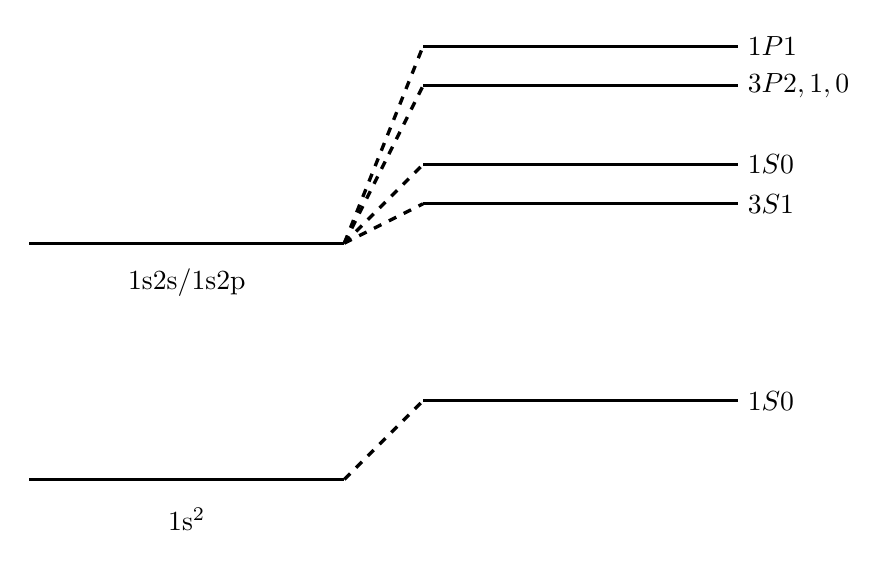
\begin{tikzpicture}
            \tikzstyle{energy level} = [very thick]
            \foreach \y in {0, 3} {
                \draw[energy level] (0, \y) -- (4, \y);
            }
            \draw[energy level] (5, 1) -- (9, 1);
            \draw[energy level, dashed] (4, 0) -- (5, 1);
            \node[right] at (9, 1) {\(\termNotation{1}{S}{0}\)};
            \foreach \y/\term in {3.5/\termNotation{3}{S}{1}, 4/\termNotation{1}{S}{0}, 5/\termNotation{3}{P}{2,1,0}, 5.5/\termNotation{1}{P}{1}} {
                \draw[energy level] (5, \y) -- (9, \y);
                \draw[energy level, dashed] (4, 3) -- (5, \y);
                \node[right] at (9, \y) {\(\term\)};
            }
            \node at (2, -0.5) {\(\mathrm{1s^2}\)};
            \node at (2, 2.5) {\(\mathrm{1s2s/1s2p}\)};
        \end{tikzpicture}
        \caption{The effect of Coulomb repulsion on the helium spectrum. Notice that this shows two possible excited states, 1s2s and 1s2p.}
        \label{fig:helium spectrum excited states}
    \end{figure}
    
    \subsection{Multi-Electron Atoms}
    Consider now a generic atom with a nuclear charge of \(Ze\) and \(N\) electrons.
    As usual we assume the nucleus is infinitely heavy and neglect all interactions apart from the Coulomb interactions.
    The Hamiltonian for this system is
    \[\operator{H} = \sum_{i=1}^{N}\left[\frac{\operator{P}_i}{2m} - \frac{Ze^2}{4\pi\varepsilon_0r_i}\right] + \sum_{i > j = 1}^{N} \frac{e^2}{4\pi\varepsilon_0 r_{ij}}.\]
    Here \(r_{ij} = \abs{\vv{r_i} - \vv{r_j}}\).
    Notice that the final sum simply sums over pairs of electrons without double counting.
    The goal is to solve the \gls{tise} but as is often the case this isn't possible so we approximate.
    
    One way of approximating is called the central field approximation.
    We treat each electron as an independent particle moving in a central potential which is a function of \(r\), the distance from the nucleus (which is assumed to be a point mass).
    The task is to come up with a potential that approximates the true potential.
    We start by considering the limiting cases of \(r \to 0\) and \(r \to \infty\).
    In the limit of \(r \to 0\) there will be no other electrons nearby and therefore we expect the only potential to be the interaction between the nucleus and electron:
    \[\lim_{r\to 0} V(r) = -\frac{Ze^2}{4\pi\varepsilon_0r}.\]
    In the limit that \(r\to\infty\) we expect all of the other \(N - 1\) electrons to be between the electron and the nucleus diluting the effective potential:
    \[\lim_{r\to\infty} V(r) = -\frac{[Z - N + 1]e^2}{4\pi\varepsilon_0 r}.\]
    Finding the intermediate form of \(V\) is not easy and is generally done by an iterative process called the Hartree--Fock method or the self-consistent field method.
    We will not discuss this here.
    
    We write the full Hamiltonian as
    \[\operator{H} = \operator{H}_c + \operator{H}'\]
    where \(\operator{H}_c\) corresponds to the central field approximation:
    \[\operator{H}_c = \sum_{i=1}^{N} \left[\frac{\operator{P}_i^2}{2m} + V(r_i)\right] = \sum_{i=1}^{N} \operator{H}_i\]
    where
    \[\operator{H}_i = \frac{\operator{P}_i^2}{2m} + V(r_i).\]
    \(\operator{H}'\) is the rest of the Hamiltonian.
    
    Considering only the central field Hamiltonian we can view it as the sum of \(N\) single particle Hamiltonians, \(\operator{H}_i\), which will have energy eigenfunctions satisfying
    \[\operator{H}_i u_{n_i\ell_im_{\ell_i}}(\vv{r_i}) = E_{n_i\ell_i}u_{n_i\ell_im_{\ell_i}}(\vv{r_i}).\]
    The energy eigenvalues are independent of \(m_{\ell_i}\) due to the spherical symmetry of \(\operator{H}_i\) but they depend on \(\ell_i\).
    The fact that the Hydrogen energy levels \emph{don't} depend on \(\ell\) turns out to be an exception rather than a rule.
    The spherical symmetry of the single particle Hamiltonians means we can decompose the energy eigenstates as
    \[u_{n_i\ell_im_{\ell_i}}(\vv{r_i}) = R_{n_i\ell_i}(r_i)Y_{\ell_i}^{m_{\ell_i}}(\vartheta_i, \varphi_i).\]
    We can then account for spin by including a spin term, \(\chi_{s_im_{s_i}}\) where, since these are single electrons \(s_i = 1/2\) and so \(m_{s_i} = \pm 1/2\).
    So the total wave function is
    \[u_{n_i\ell_im_{\ell_i}s_im_{s_i}}(i) = u_{n_i\ell_im_{\ell_i}}(\vv{r_i}) \tensorProd \chi_{s_im_{s_i}}.\]
    The total energy of the atom in this approximation is simply the sum of the individual energies:
    \[E_c = \sum_{i=1}^{N} E_{n_i\ell_i}.\]
    The wave function for the entire system is totally antisymmetric, as spin statistics demands, and is a linear combination of single electron spin orbitals given by the Slater determinant:
    \[
        \Psi(1, 2, \dotsc, N) = \frac{1}{\sqrt{N!}} 
        \begin{vmatrix}
            u_\alpha(1) & u_\beta(1) & \dotsc & u_\nu(1)\\
            u_\alpha(2) & u_\beta(2) & \dotsc & u_\nu(2)\\
            \vdots      & \vdots     & \ddots & \vdots\\
            u_\alpha(N) & u_\beta(N) & \dotsc & u_\nu(N)\\
        \end{vmatrix}
    \]
    Here \(\alpha\), \(\beta\) and \(\nu\) represent different sets of the four quantum numbers \((n, \ell, m_\ell, m_s)\) so that the final state satisfies the Pauli exclusion principle.
    
    The order of the individual energy levels doesn't depend on the potential.
    The order is
    \[\mathrm{1s2s2p3s3p[4s3d]4p[5s4d]5p[6s4f5d]}.\]
    Orbitals in square brackets are close enough in energy that the exact order can change from atom to atom.
    Electrons with the same value of \(n\) are said to be in the same shell, electrons with the same values of \(n\) and \(\ell\) are said to be in the same sub shell.
    The maximum number of electrons in the same subshell is \(2(2\ell + 1)\).
    The electron configuration of a given atom is given using a superscript to denote the number of electrons in a given subshell.
    For example in its ground state carbon has the electron configuration \(1s^22s^22p^2\) which can also be written as \([\ce{He}]\mathrm{2s^22p^2}\) where \([\ce{He}]\) denotes the electron configuration of helium in its ground state which is \(\mathrm{1s^2}\).
    
    \section{Variational Methods}
    \subsection{The Theory}
    Variational methods, also known as Rayleigh--Ritz methods, are a way of approximating the ground state energy of a given Hamiltonian, \(\operator{H}\).
    Suppose \(\operator{H}\) has a complete set of eigenstates, \(\{\ket{n}\}\), and corresponding energy eigenvalues, \(\{E_n\}\), such that \((E_n)\) is an increasing sequence, that is
    \[E_1 \le E_2 \le \dotsb \le E_{i} \le E_{i + 1} \le \dotsb\]
    Then we can expand any state, \(\ket{\psi}\), as a linear superposition of these states as
    \[\ket{\psi} = \sum_n c_n\ket{\psi}, \qquad\text{where}\qquad c_n = \braket{n}{\psi}.\]
    The expectation energy of a system in state \(\ket{\psi}\) is then
    \[\expected{E} = \frac{\bra{\psi}\operator{H}\ket{\psi}}{\braket{\psi}{\psi}} = \frac{\sum_n\abs{c_n}^2E_n}{\sum_n \abs{c_n}^2} \ge \frac{\sum_n \abs{c_n}^2 E_1}{\sum_n \abs{c_n}^2} = E_1.\]
    Where we have used the ordering of \((E_n)\) to replace all \(E_n\) with \(E_1 \le E_n\).
    We see that \(\expected{E}\) provides an upper bound for the ground state energy, \(E_1\).
    Using this fact the variational method simply gives us a way to find a close upper bound.
    
    To apply the variational method to a given Hamiltonian, \(\operator{H}\), choose a trial state, \(\ket{\psi_T}\), which depends on the parameters \(\alpha_1, \dotsc, \alpha_r\).
    We then calculate
    \[E(\alpha_1, \dotsc, \alpha_r) = \frac{\bra{\psi_T}\operator{H}\ket{\psi_T}}{\braket{\psi_T}{\psi_T}}.\]
    To find the upper bound on the ground state energy we then minimise \(E\) with respect to its parameters by finding \(\{\alpha_i^*\}\) such that
    \[\pdvat{E}{\alpha_i}{\alpha_i^*} = 0.\]
    This then gives us a best estimate for the upper bound of the ground state energy.
    
    This method works best when \(\ket{\psi_T}\) is as close to the true ground state as possible.
    This means we should consider symmetry requirements when choosing \(\ket{\psi_T}\).
    For example if our system is a particle in a box we should choose \(\psi_T(\vv{r})\) to be zero at the boundaries.
    
    It is important to note that the only thing variational methods predict is an upper bound of the ground state energy.
    The resulting trial state, \(\ket{\psi_T}\), may have a close value for the expectation value of the energy but there is no reason why it should be close to the ground state.
    Similarly if we choose our parameters, \(\{\alpha_i\}\), to have some physical meaning we shouldn't read too much into whatever values they have.
    
    \subsection{Hydrogen Ground State}
    Suppose we want to use variational methods to estimate the ground state energy of hydrogen.
    After various symmetry considerations we conclude that the ground state will have \(\ell = 0\) which means the radial part of the wave function, \(Y_\ell^m\), will be spherically symmetric.
    Thus we choose our trial solution to be the radial component of the wave function.
    Further \(\ell = 0\) is the only value where the radial component doesn't need to vanish at the origin.
    The only requirement is that our function be square integrable on \([0, \infty)\), i.e. \(\psi_T\in \squareIntegrable([0, \infty)\).
    One such function is
    \[\psi_T(r) = Ce^{-\alpha r}\]
    where \(C\) is a normalisation constant and \(\alpha\) is a variational parameter (not the fine structure coefficient).
    Notice that this is actually the form of the true wave function for the ground state.
    
    First we will normalise \(\ket{\psi_T}\) to avoid constant factors of \(1/\braket{\psi_T}{\psi_T}\).
    \begin{align*}
        \braket{\psi_T}{\psi_T} &= \int_V \psi_T^*(r)\psi_T(r) \dd{V}\\
        &= \abs{C}^2 \int_{0}^{2\pi} \dd{\varphi} \int_{0}^{\pi} \dd{\vartheta} \int_{0}^{\infty} \dd{r} e^{-2\alpha r}r^2\sin\vartheta\\
        &= \abs{C}^2\int_0^{2\pi}\dd{\varphi} \int_0^{\pi} \sin\vartheta \dd{\vartheta} \int_0^{\infty} r^2e^{-2\alpha r} \dd{r}\\
        &= \abs{C}^2\cdot2\pi\cdot 2 \cdot \left(\left[-\frac{1}{2\alpha} r^2e^{-2\alpha r}\right]_0^{\infty} + \frac{1}{\alpha}\int_0^{\infty} re^{-2\alpha r} \dd{r}\right)\\
        &= 4\pi\abs{C}^2 \frac{1}{\alpha} \int_0^{\infty} re^{-2\alpha r} \dd{r}\\
        &= 4\pi\abs{C}^2 \frac{1}{\alpha} \left(\left[-\frac{1}{2\alpha} re^{-2\alpha r}\right]_0^{\infty} + \frac{1}{2\alpha} \int_0^{\infty} e^{-2\alpha r} \dd{r}\right)\\
        &= 4\pi\abs{C}^2\frac{1}{2\alpha^2} \int_0^{\infty} e^{-2\alpha r} \dd{r}\\
        &= 4\pi\abs{C}^2\frac{1}{2\alpha^2} \left[-\frac{1}{2\alpha}e^{-\alpha r}\right]_0^{\infty}\\
        &= \pi\abs{C}^2\frac{1}{\alpha^3}
    \end{align*}
    For this to equal 1 we must have \(C = \sqrt{\alpha^3/\pi}\).
    
    The expectation value is linear so we can find \(\expected{\operator{H}}\) using
    \[\expected{\operator{H}} = \expected{\operator{T} + \operator{V}} = \expected{\operator{T}} + \expected{\operator{V}}.\]
    We will start with \(\expected{\operator{V}}\).
    \begin{align*}
        \expected{\operator{V}} &= \bra{\psi_T} \operator{V} \ket{\psi_T}\\
        &= -\frac{\abs{C}^2e^2}{4\pi\varepsilon_0} \int_V\frac{1}{r}e^{-2\alpha r} \dd{V}\\
        &= -\frac{\abs{C}^2e^2}{4\pi\varepsilon_0} \int_0^{2\pi}\dd{\varphi} \int_0^\pi \dd{\vartheta} \int_0^\infty \dd{r} \frac{1}{r}e^{-2\alpha r} r^2\sin\vartheta\\
        &= -\frac{\abs{C}^2e^2}{\varepsilon_0} \int_0^\infty re^{-2\alpha r} \dd{r}\\
        &= -\frac{\abs{C}^2e^2}{\varepsilon_0} \left(\left[-\frac{1}{2\alpha} re^{-2\alpha r}\right]_0^{\infty} + \frac{1}{2\alpha} \int_0^{\infty} e^{-2\alpha r} \dd{r} \right)\\
        &= -\frac{\abs{C}^2e^2}{\varepsilon_0} \frac{1}{2\alpha} \int_0^{\infty} e^{-2\alpha r} \dd{r}\\
        &= -\frac{\abs{C}^2e^2}{\varepsilon_0}\frac{1}{2\alpha} \left[-\frac{1}{2\alpha} e^{-2\alpha r}\right]_0^{\infty}\\
        &= -\frac{1}{4\alpha^2}\frac{\abs{C}^2e^2}{\varepsilon_0}\\
        &= -\frac{\alpha e^2}{4\pi\varepsilon_0}
    \end{align*}
    Next we find the expectation value of the energy of the kinetic energy.
    To do this we will use the following identity:
    \[\div(f \vv{v}) = f(\div\vv{v}) + (\grad f)\cdot\vv{v}.\]
    Considering the particular case \(f = \varphi^*\) and \(\vv{v} = \grad\varphi\) this becomes
    \[\div(\varphi^*\grad\varphi) = \varphi^*(\div(\grad\varphi)) + (\grad\varphi^*) \cdot (\grad\varphi).\]
    Integrating over all space this becomes
    \[\int_V \div(\varphi^*\grad\varphi) \dd{V} = \int_V \varphi^*\laplacian\varphi \dd{V} + \int_V (\grad\varphi^*)\cdot(\grad\varphi) \dd{V}.\]
    Using the divergence theorem the left hand side becomes
    \[\int_V \div(\varphi^*\grad\varphi) \dd{V} = \int_S (\varphi^*\grad\varphi)\cdot\dd{\vv{S}}.\]
    If we take \(V\) to be all of space then the boundary, \(S\), is at infinity.
    Since we are assuming \(\varphi\in\squareIntegrable(\reals^3)\) it will be zero when evaluated at infinity so the left hand side of the identity disappears and we are left with
    \[\int_V \varphi^*\laplacian\varphi \dd{V} = -\int_V \abs{\grad\varphi}^2\dd{V}.\]
    The expectation value of the the kinetic energy is then
    \begin{align*}
        \expected{\operator{T}} &= \frac{1}{2m} \bra{\psi_T} \operator{P}^2 \ket{\psi_T}\\
        &= -\frac{\hbar^2}{2m} \int_V \psi_T^* \laplacian \psi_T \dd[3]{r}\\
        &= \frac{\hbar^2}{2m} \int_V \abs{\grad\psi_T}^2\dd[3]{r}
    \end{align*}
    The trial function, \(\psi_T\), depends only on \(r\) so
    \[\grad\psi_T = \pdv{\psi_T}{r} \ve{r}\]
    and hence
    \[\abs{\grad\psi_T}^2 = \abs{\pdv{\psi_T}{r}} = \alpha^2\abs{\psi_T}^2.\]
    So
    \[\expected{\operator{T}} = \frac{\hbar^2\alpha^2}{2m}.\]
    So the expectation value of the Hamiltonian is
    \[E(\alpha) = \expected{\operator{H}} = \expected{\operator{T}} + \expected{\operator{V}} = \frac{\hbar^2\alpha^2}{2m} - \frac{e^2\alpha}{4\pi\varepsilon_0}.\]
    Differentiating with respect to \(\alpha\) we have
    \[\pdv{E}{\alpha} = \frac{\hbar^2\alpha}{m} - \frac{e^2}{4\pi\varepsilon_0}.\]
    Demanding that this is zero so \(E\) is minimised we have
    \[\alpha = \frac{me^2}{r\pi\varepsilon_0\hbar^2} = \frac{1}{a_0}\]
    where \(a_0\) is the Bohr radius.
    Thus an upper bound on the ground state energy is
    \[E = -\frac{e^2}{2(4\pi\varepsilon_0)a_0} = \SI{-1}{\rydberg} = \SI{-13.6}{\electronvolt}.\]
    This is actually the ground state energy because our trial function with \(\alpha = 1/a_0\) is the ground state eigenfunction so \(\expected{\operator{H}}\) is simply the expectation value of the energy of a particle in a ground state, which is the ground state energy.
    
    \subsection{Helium Ground State}
    Suppose we want to use variational methods to calculate the ground state energy of helium.
    As a trial wave function we take a product of 1s orbital wave functions with an effective nuclear charge \(\tilde{Z}\) which accounts for shielding of the nucleus by the other electron.
    \[\psi_T(r_1, r_2) = \frac{\tilde{Z}^3}{\pi a_0^3} \exp\left[-\frac{\tilde{Z}}{a_0}(r_1 + r_2)\right].\]
    Setting \(\tilde{Z} = Z\) would be the equivalent of no electron-electron interaction.
    The variational parameter in this wave function is \(\tilde{Z}\).
    
    For the kinetic energy we can use the same result as for hydrogen:
    \[\expected{\operator{T}} = -\frac{\hbar^2}{2m}\ket{\psi_T}(\operator{P}_1^2 + \operator{P}_2^2)\ket{\psi_T} = \frac{\hbar^2 \tilde{Z}^2}{ma_0^2} = 2\tilde{Z}^2\,\si{\rydberg}.\]
    Similarly for the potential energy
    \[\expected{\operator{V}} = -\frac{2Ze^2}{4\pi\varepsilon_0a_0} \tilde{Z} = -4Z\tilde{Z}\,\si{\rydberg}.\]
    Finally the electron-electron Coulomb term has an expectation value of \(5/4\tilde\,\si{\rydberg}\).
    The total energy is then
    \[E(\tilde{Z}) = 2\left[\tilde{Z}^2 - \left(2Z - \frac{5}{8}\right)\tilde{Z}\right] \,\si{\rydberg}.\]
    Differentiating with respect to \(\tilde{Z}\), setting equal to zero, and then rearranging gives us
    \[\tilde{Z} = Z - \frac{5}{16}.\]
    The energy corresponding to this is then
    \[E(\tilde{Z}) = \SI{-5.695}{\rydberg} = \SI{-77.46}{\electronvolt}.\]
    This is within \SI{2}{\percent} of the measured value of \(\SI{-78.975}{\electronvolt}\) and is better than the first order perturbation result of \(\SI{-74.8}{\electronvolt}\).
    
    \subsection{Excited States}
    It is sometimes possible to use variational methods to find upper bounds on excited states.
    Suppose we know enough about the ground state to choose a trial state that is orthogonal to the ground state such that \(\braket{n=1}{\psi_T} = 0\).
    Then the expansion of \(\ket{\psi_T}\) in \(\{\ket{n}\}\) doesn't contain \(\ket{n=1}\) and so
    \[\frac{\bra{\psi_T}\operator{H}\ket{\psi_T}}{\braket{\psi_T}{\psi_T}} = \frac{\sum_{n=2}\abs{c_n}^2E_n}{\sum_{n=2} \abs{c_n}^2} \ge E_2.\]
    Using variational methods as before we can then find an upper bound on \(E_2\).
    
    The problem with this is we don't typically know the eigenstates so we can't construct an orthogonal state.
    We can avoid this problem if we are interested in an excited state with symmetries lower energy states don't posses.
    If we choose a trial state that does have these symmetries then it is guaranteed to be orthogonal to the lower energy states and we can use variational methods.
    
    Consider, for example, helium.
    It's ground state is a \(\termNotation{1}{S}{}\) state.
    The first four excited states are \(\termNotation{3}{S}{}\), \(\termNotation{1}{S}{}\), \(\termNotation{3}{P}{}\), and \(\termNotation{1}{P}{}\) states/
    Apart from the \(\termNotation{1}{S}{}\) state these all have symmetries different from the ground state.
    For example \(\termNotation{}{P}{}\) states have \(L = 1\) and are therefore orthogonal to the ground state which has \(L = 0\).
    A trial function that may be considered when trying to find an upper bound on the state 1s2p is
    \[\psi_T^{\pm}(\vv{r_1}, \vv{r_2}) = C_{\pm} [f(r_1)g(r_2)\cos\vartheta_1 \pm f(r_2)g(r_2)\cos\vartheta_2]\]
    where
    \[f(r) = e^{-\alpha r / a_0}, \qquad\text{and}\qquad g(r) = re^{-\beta r/ 2a_0}.\]
    This has two variational parameters \(\alpha\) and \(\beta\).
    